\documentclass[titlepage,a4paper,12pt]{report}
\usepackage{amssymb,amsfonts,amsmath}
\usepackage{fullpage}
\usepackage{graphicx}
%\usepackage[cc]{titlepic}
\usepackage{amsthm}
\newtheorem{definition}{Definition}[section]
\newtheorem{example}{Example}[section]
\newtheorem{theorem}{Theorem}[section]
\newtheorem{exercise}{Exercise}[section]
\newtheorem{corollary}{Corollary}[section]
\newtheorem{proposition}{Proposition}[section]
\pdfpagewidth 8.5in
\pdfpageheight 11in
\setlength\topmargin{-0.5in}
\setlength\headheight{0in}
\setlength\headsep{0in}
\setlength\textheight{9.5in}
\setlength\textwidth{7.0in}
\setlength\oddsidemargin{-0.5in}
\setlength\evensidemargin{1.0in}
\setlength\parindent{0.25in}
\setlength\parskip{0.25in}
%\begin{titlepage}
%\usepackage{titlepic}
%\titlepic{
\includegraphics[width=0.2\textwidth]{uz1.png}}
%
%\title{\textbf{HMTH111 Calculus 2}}
%\author{Nhawu. G\\
%		Department of Mathematics\\
%		University of Zimbabwe, ZIM}
%
%\end{titlepage}

\begin{document}
\begin{titlepage}
 
\begin{center}
 
 
% Upper part of the page

\includegraphics[width=0.15\textwidth]{uz1.png}\\[1cm]
 
\textsc{\LARGE University of Zimbabwe}\\[1.5cm]
 
\textsc{\Large HMTHCS111 CALCULUS 2}\\[0.5cm]
 
 
% Title

{ \huge \bfseries Calculus of Several Variables}\\[0.4cm]
 

 
% Author and supervisor
\begin{minipage}{0.4\textwidth}
\begin{center} \large
\emph{Author:}\\
G. \textsc{Nhawu}
\end{center}
\end{minipage}
\begin{minipage}{0.4\textwidth}
\begin{flushright} \large
\emph{Department:} \\
\textsc{Mathematics and Computational Sciences}
\end{flushright}
\end{minipage}

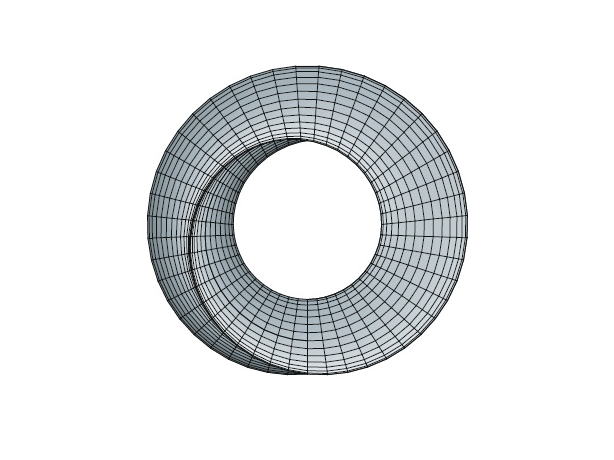
\includegraphics[width=0.7\textwidth]{umblictorus.png}\\[1cm]
 \vfill
 
 
% Bottom of the page
{\large \today}
 
\end{center}
 
\end{titlepage}
%\maketitle
\tableofcontents
\setcounter{chapter}{1}
\chapter{Vectors and the Geometry of Space}
\begin{center}
	\small{\parbox{18cm}{
		\begin{raggedright}
		{\small
		\textit{Don't be pushed around by the fears in your mind. Be led by the dreams in your heart.}
 }
 
				\vspace{.5cm}\hfill{---Roy T. Bennett, The Light in the Heart.}
		\end{raggedright}
	}
} 
\end{center}
A vector is a quantity that is characterized by \textbf{magnitude} and \textbf{direction}. We also use the term \textbf{length} for magnitude. A scalar, on the other hand, is a quantity which has \textbf{magnitude} only. To differentiate the types of quantities, let's consider a typical vector, \textbf{displacement} or \textbf{change of position}. In order to specify displacement, we need to know two things: \textit{how far?} and \textit{in what direction?} In other words, we need to specify \textbf{distance} and the \textbf{direction}. Thus we see that distance is a scalar whereas displacement is a vector.

\noindent Consider the following two situations:
\begin{enumerate}
\item A complete stranger to Zimbabwe is in Harare and wants to travel to Masvingo. Is it sufficient to simply tell them that Masvingo is 350 kilometers from Harare?
\item A well-informed Zimbabwean wants to travel from Harare to Masvingo. Will it be sufficient to tell them that Masvingo is 350 kilometers from Harare?
\end{enumerate}
Clearly, the information in the first case is not sufficient as the stranger would also want to know the direction in which to travel. However, in the second case, it is assumed that the person already has some idea of the location of Masvingo relative to Harare and so specifying \textbf{only} distance would suffice.

\noindent The following are examples of vectors: force, displacement, acceleration, momentum and  velocity . However, the following quantities are scalars and not vectors: area, volume, distance, speed, energy, work, electrical resistance, temperature, mass and time.
%Many quantities in geometry and physics, such as area, volume,energy, work, electrical resistance, temperature, mass and time, can be characterized by single real numbers scaled to appropriate units of measure. We call these \textbf{scalar quantities}, and the real number associated with each is called a \textbf{scalar}. A scalar quantity has magnitude, including the sense of being positive or negative, but no assigned position and no assigned direction.

%\noindent Other quantities such as force, displacement, acceleration, momentum and  velocity involve both magnitude and direction and cannot be characterized by single real numbers. A \textbf{vector} is a quantity having both magnitude and direction.
\section{Basic Definitions and Notation}
\noindent Graphically a vector is represented by an arrow $\overrightarrow{OP}$ defining
the direction, the magnitude of the vector being indicated by
the length of the arrow. The tail end $O$ of the arrow is called the
\textit{origin} or \textit{initial point} of the vector, and the head $P$ is called the \textit{terminal point} or \textit{terminus}. This arrow representing the vector is called a \textit{directed line segment}. The length $|\overrightarrow{OP}|$  is the magnitude of the line segment from $O$ to $P$. 
\begin{figure}[h!]
\input{notes.pic}
\caption{Directed line segment}
\end{figure}

\noindent Vectors can be represented in text by bold-case letters, such as $\textbf{A, B, C}$ and so on or lower-case boldface letters such as $\textbf{a, b, c}$ and so on. When written by hand, however, vectors are often denoted by letters with arrows above them, such as $\overrightarrow{a}, \overrightarrow{b}$ and so on or a bar above, such as $\overline{a}, \overline{ b}$ and so on or a bar below, such as $\underline{a}, \underline{b}$ and so on. When the initial point of the vector is fixed, it is called a \textbf{fixed} or \textbf{localized} vector, otherwise, it is a free vector.

\section{Unit Vectors}
A \textbf{unit vector} is a vector of unit length. A unit vector is sometimes denoted by $\widehat{e}$ or $\widehat{\bf{e}}$ . Therefore,
\[|\widehat{\bf{e}}| =1.\] Any vector can be made into a unit vector by dividing it by its length, that is, 
\[\widehat{\bf{e}}=\dfrac{\bf{u}}{|\bf{u}|}.\] So $\dfrac{\bf{u}}{|\bf{u}|}$ is a unit vector in the direction of the vector $\textbf{u}$.

\noindent In three-dimensional space $\mathbb{R}^3$, we denote the unit vectors in the positive \textit{x}-axis, positive \textit{y}-axis and positive \textit{z}-axis by \textbf{i}, \textbf{j}, \textbf{k} respectively. Thus the position vector of a point $(x,y,z)$ is
\begin{eqnarray}
x\textbf{i}+y\textbf{j}+z\textbf{k}.\nonumber
\end{eqnarray}
In a similar way, the position vector \textbf{r} of a point $(x,y)$ in two-dimensional space $\mathbb{R}^2$ is 
\begin{eqnarray}
x\textbf{i}+y\textbf{j}. \nonumber
\end{eqnarray}
In the notation above, the numbers \textit{x}, \textit{y}, \textit{z} are the \textbf{components} of the vectors.

\noindent We also denote vectors in $\mathbb{R}^3$ and $\mathbb{R}^2$ using \textbf{column vectors}. For example the vector $x\textbf{i}+y\textbf{j}+z\textbf{k}$ in $\mathbb{R}^3$ is denoted by $\begin{pmatrix}
x\\
y\\
z
\end{pmatrix}$ and the vector $x\textbf{i}+y\textbf{j}$ in $\mathbb{R}^2$ is denoted by $\begin{pmatrix}
x\\
y
\end{pmatrix}$.
%\noindent An important set of unit vectors are those having the directions of the positive $x$, $y$, and $z$ axes of a three dimensional rectangular coordinate system. Vectors will be denoted as 
%\[\textbf{A}=(A_1, A_2, A_3)=A_1\textbf{i}+A_2\textbf{j}+A_3{\textbf{k}},\] where $\bf{i}, \bf{j}$ and $\bf{k}$ are unit base vectors defined by 
%\[{\bf{i}}= (1,0,0), \quad {\bf{j}}=(0,1,0) \quad \mbox{and} \quad {\bf{k}}=(0,0,1).\]The vectors $A_1{\bf{i}}, A_2{\bf{j}}$, and $A_3{\bf{k}}$ are called the \textbf{rectangular component vectors} or simply \textbf{component vectors} of $\textbf{A}$ in the $x$, $y$ and $z$ directions respectively. $A_1, A_2$ and ${A}_3$ are called the rectangular components or simply components of $\bf{A}$ in the $x, y$ and $z$ directions respectively.
\section{Magnitude or Length of a Vector}
The magnitude or length of a vector $\textbf{r}$ is denoted by $|\textbf{r}|$. If a vector $\textbf{r}=x\textbf{i}+y\textbf{j}+z\textbf{k}$, then it can be easily shown by use of Pythagoras' theorem that
\[|{\bf{r}}|=\sqrt{x^2+y^2+z^2}.\] For example if $\textbf{r}=\textbf{i}-2\textbf{j}+2\textbf{k}$, then the magnitude $|\textbf{r}|=\sqrt{1^2+(-2)^2+2^2}=\sqrt{1+4+4}=\sqrt{9}=3$. 
%In particular, the \textbf{position vector} or \textbf{radius vector} $\bf{r}$ from $O$ to the point $(x,y,z)$ is written as \[\textbf{r}=x\textbf{i}+y\textbf{j}+z\textbf{k}\] and has magnitude $r=|\textbf{r}|=\sqrt{x^2+y^2+z^2}$. That is, $\bf{i}, \bf{j}$ and $\bf{k}$ are three mutually perpendicular vectors pointing along $Ox, Oy$ and $Oz$ axes respectively. These vectors are often called the \textbf{basis vectors}. 
\begin{example}
Given ${\bf{A}}=3{\bf{i}}-2{\bf{j}}+{\bf{k}}, {\bf{B}}=2{\bf{i}}-4{\bf{j}}-3{\bf{k}}$ and ${\bf{C}}=-{\bf{i}}+2{\bf{j}}+2{\bf{k}}$, find the magnitudes of (i)\, ${\bf{C}}$, \quad (ii)\, ${\bf{A}}+{\bf{B}}+{\bf{C}}$ and (iii)\, $2{\bf{A}}-2{\bf{B}}-5{\bf{C}}$.

\noindent \textbf{Solution:}\,  (i)\, $|{\bf{C}}|=|-{\bf{i}}+2{\bf{j}}+2{\bf{k}}|=\sqrt{(-1)^2+2^2+2^2}=3$.\\
(ii)\, ${\bf{A}}+{\bf{B}}+{\bf{C}}=3{\bf{i}}-2{\bf{j}}+{\bf{k}} +2{\bf{i}}-4{\bf{j}}-3{\bf{k}}-{\bf{i}}+2{\bf{j}}+2{\bf{k}} =(3+2-1){\bf{i}}+(-2-4+2){\bf{j}}+(1-3+2){\bf{k}}=4{\bf{i}}-4{\bf{j}}+0{\bf{k}}$. Then $|{\bf{A}}+{\bf{B}}+{\bf{C}}|=|4{\bf{i}}-4{\bf{j}}+0{\bf{k}}|=\sqrt{4^2+(-4)^2}=\sqrt{32}=4\sqrt{2}$.\\
(iii)\, $2{\bf{A}}-3{\bf{B}}-5{\bf{C}}=2(3{\bf{i}}-2{\bf{j}}+{\bf{k}})-3(2{\bf{i}}-4{\bf{j}}-3{\bf{k}})-5(-{\bf{i}}+2{\bf{j}}+2{\bf{k}})$
$=5{\bf{i}}-2{\bf{j}}+{\bf{k}}$. Then $|2{\bf{A}}-2{\bf{B}}-5{\bf{C}}| =|5{\bf{i}}-2{\bf{j}}+{\bf{k}}|=\sqrt{5^2+(-2)^2+1^2}=\sqrt{30}$.
\end{example}
\begin{example}
Find the component form and magnitude of the vector ${\bf{A}}$ having initial point $(-2,3,1)$ and terminal point $(0,-4,4)$. Then find a unit vector in the direction of ${\bf{A}}$.

\noindent \textbf{Solution:} The component form of ${\bf{A}}$ is 
\[{\bf{A}}=(0-(-2), -4-3, 4-1)=(2,-7,3)\] which implies that its magnitude is 
\[|{\bf{A}}|=\sqrt{2^2+(-7)^2+3^2}=\sqrt{62}.\] The unit vector in the direction of ${\bf{A}}$ is 
\[{\bf{U}}=\dfrac{{\bf{A}}}{|{\bf{A}}|}=\dfrac{1}{\sqrt{62}}(2,-7,3)=\left(\dfrac{2}{\sqrt{62}}, \dfrac{-7}{\sqrt{62}}, \dfrac{3}{\sqrt{62}}\right).\]
\end{example}
\section{Parallel Vectors}
Two non-zero vectors ${\bf{A}}$ ans ${\bf{B}}$ are \textbf{parallel} if there is some scalar $c$ such that ${\bf{A}}=c{\bf{B}}$.
\begin{example}
Vector ${\bf{A}}$ has initial point $(2,-1,3)$ and terminal point $(-4,7,5)$. Which of the following vectors is parallel to ${\bf{A}}$? (i)\, ${\bf{B}}=(3,-4,-1)$ and (ii)\, ${\bf{C}}=(12,-16,4)$.

\noindent \textbf{Solution:} Writing ${\bf{A}}$ in component form
\[{\bf{A}}=(-4-2, 7-(-1), 5-3)=(-6,8,2).\]
(i)\, Because ${\bf{B}}=(3,-4,-1)=-\frac{1}{2}(-6,8,2)=-\frac{1}{2}{\bf{A}}$, then ${\bf{B}}$ is parallel to ${\bf{A}}$.\\
(ii)\, In this  case, you want to find a scalar $c$ such that 
\begin{eqnarray*}
(12,-16,4) &=& c(-6,8,2)\\
12=-6c & \Rightarrow & c=-2 \\
-16 =8c & \Rightarrow & c=-2 \\
4=2c & \Rightarrow & c=2.
\end{eqnarray*}
Because there is no $c$ for which the equation has a solution, the vectors are not parallel.
\end{example}
\noindent \textbf{Definition}\\
Two or more vectors are said to be collinear vectors, when they are along the same lines or parallel lines.\\
\begin{theorem}
Let \textbf{a} and \textbf{b} be non-zero and non-collinear vectors. Then $x\textbf{a}+y\textbf{b}=0$ implies that $x=y=0$.
\end{theorem}
\begin{proof}
Suppose $x\textbf{a}+y\textbf{b}=0$ where $x\neq 0$. This means that $\textbf{a}=-(\frac{y}{x})\textbf{b}$. Thus the vectors \textbf{a} and \textbf{b} are parallel. In other words they are parallel to the same line or are collinear. Contradiction. Hence $x$ must be equal to zero and so $y\textbf{b}=0$. Therefore $y=0$ as $\textbf{b}\neq 0$.
\end{proof}
\begin{theorem}
Let \textbf{a} and \textbf{b} be non-zero and non-collinear vectors. Then $x_1\textbf{a}+y_1\textbf{b}=x_2\textbf{a}+y_2\textbf{b}$ implies that $x_1=x_2$ and $y_1=y_2$.
\end{theorem}
\noindent The proof of this theorem is left as an exercise for you.

\section{Vector Algebra}
The operations of addition, subtraction and multiplication familiar in the algebra
of numbers or scalars are, with suitable definition, capable of extension
to an algebra of vectors. The following definitions are fundamental.
\begin{itemize}
\item[(i)] Two vectors $\textbf{A}$ and $\textbf{B}$ are \textit{equal} if they have the same magnitude and direction regardless of the position of their initial points. 
\item[(ii)] A vector having direction opposite to that of vector $\textbf{A}$ but having the same magnitude is denoted by $\textbf{-A}$.
\item[(iii)] The \textbf{sum} or \textbf{resultant} of vectors $\bf{A}$ and $\bf{B}$ is a vector $\bf{C}$ formed by placing the initial point of $\bf{B}$ on the terminal point of $\bf{A}$ and then joining the initial point of $\bf{A}$ to the terminal point of $\bf{B}$. This sum is written $\bf{A}+\bf{B}$, i.e. $\bf{C} = \bf{A}+\bf{B}$. 
\begin{figure}[h!]
\input{bold.pic}
\caption{${\bf{A}}+{\bf{B}}={\bf{C}}$}
\end{figure}
\begin{theorem}
Vector addition is commutative, that is 
\[\bf{A}+\bf{B}=\bf{B}+\bf{A},\] for each pair of vectors $\bf{A}$ and $\bf{B}$.
\end{theorem}
\begin{theorem}
Vector addition is associative, that is 
\[\bf{A}+(\bf{B}+\bf{C})=(\bf{A}+\bf{B})+\bf{C},\] for any triple of vectors $\bf{A}, \bf{B}$ and $\bf{C}$.
\end{theorem}
\item[(iv)] The \textbf{difference} of vectors $\bf{A}$ and $\bf{B}$, represented by $\bf{A} -\bf{B}$, is that vector $\bf{C}$ which added to $\bf{B}$ yields vector $\bf{A}$. Equivalently, $\bf{A}- \bf{B}$ can be defined as the sum $\bf{A} + (-\bf{B})$.

\noindent If $\bf{A} = \bf{B}$, then $\bf{A}-\bf{B}$ is defined as the \textbf{null} or \textbf{zero vector} and is represented by the symbol $\bf{0}$ or simply $0$. It has zero magnitude and no specific direction. A vector which is not
null is a \textbf{proper vector}. All vectors will be assumed proper unless otherwise stated.
\item[(v)] The \textbf{product} of a vector $\bf{A}$ by a scalar $m$ is a vector $m\bf{A}$ with magnitude $|m|$ times the magnitude of $\bf{A}$ and with direction the same as or opposite to that of $\bf{A}$, according as $m$ is positive
or negative. If $m = 0, m\bf{A}$ is the null vector.
\end{itemize}
\section{Laws of Vector Algebra}
If $\bf{A}, \bf{B}$ and $\bf{C}$ are vectors and $m$ and $n$ are scalars, then
\begin{itemize}
\item[(i)] $\bf{A}+\bf{B}=\bf{B}+\bf{A}$ \quad \quad \quad \quad \quad \quad  Commutative Law for Addition.
\item[(ii)] $\bf{A}+(\bf{B}+\bf{C})=(\bf{A}+\bf{B})+\bf{C}$ \quad Associative Law of Addition.
\item[(iii)] $m(n{\bf{A}})=mn{\bf{A}}=n(m{\bf{A}})$ \quad \quad Associative Law for Multiplication.
\item[(iv)] $(m+n){\bf{A}}=m{\bf{A}}+n{\bf{A}}$ \quad \quad Distributive Law.
\item[(v)] $m({\bf{A}}+{\bf{B}})=m{\bf{A}}+m{\bf{B}}$ \quad \quad Distributive Law.
\end{itemize}
\section{The Dot or Scalar Product}
So far we have studied two operations with vectors, vector addition and multiplication by a scalar, each of which yield another vector. In this section you will study a third vector operation, called the \textbf{dot product}, this product yields a scalar, rather than a vector.

\noindent The \textbf{dot} or \textbf{scalar product} of two vectors ${\bf{A}}=A_1{\bf{i}}+A_2{\bf{j}}+A_3{\bf{k}}$ and ${\bf{B}}=B_1{\bf{i}}+B_2{\bf{j}}+{B_3\bf{k}}$, denoted by ${\bf{A\cdot B}}$ (read ${\bf{A}}$ dot ${\bf{B}}$) is defined as the product of the magnitudes of ${\bf{A}}$ and ${\bf{B}}$ and the cosine of the angle $\theta$ between them, that is, 
\[{\bf{A \cdot B}}=|{\bf{A}}||{\bf{B}}|\cos \theta =A_1B_1+A_2B_2+A_3B_3\] where $0\leq \theta \leq \pi$.
\begin{example}
Given ${\bf{A}}=2{\bf{i}}+4{\bf{j}}+6{\bf{k}}$ and ${\bf{B}}={\bf{i}}-3{\bf{j}}+2{\bf{k}}$. Compute the scalar product of ${\bf{A}}$ and ${\bf{B}}$. 

\noindent \textbf{Solution:} From the definition, the scalar product is given by 
\[{\bf{A\cdot B}}=(2)\cdot (1)+(4)\cdot (-3)+(6)(2)=2-12+12=2.\]
\end{example}
\noindent The following laws are valid
\begin{itemize}
\item[(i)] ${\bf{A\cdot B}}={\bf{B\cdot A}}$ \quad \quad Commutative Law for Dot Products. 
\item[(ii)] ${\bf{A}\cdot (\bf{B}+\bf{C})}={\bf{A\cdot B}} +{\bf{A\cdot C}}$ \quad Distributive Law.
\item[(iii)] $m({\bf{A\cdot B}})=(m{\bf{A}})\cdot {\bf{B}}={\bf{A}}\cdot (m{\bf{B}})=({\bf{A\cdot B}})m,$ where $m$ is a scalar.
\item[(iv)] ${\bf{i}\cdot \bf{i}}={\bf{j}\cdot \bf{j}}={\bf{k}\cdot \bf{k}}=1$, ${\bf{i}\cdot \bf{j}}={\bf{j}\cdot \bf{k}}={\bf{k}\cdot \bf{i}}=0$.
\item[(v)] If ${\bf{A\cdot B}}=0$ and ${\bf{A}}$ and ${\bf{B}}$ are not null vectors, then ${\bf{A}}$ and ${\bf{B}}$ are perpendicular. 
\end{itemize}
\subsection{Angle Between Two Vectors}
If $\theta$ is the angle between two non-zero vectors ${\bf{A}}$ and ${\bf{B}}$, then 
\[\cos \theta =\dfrac{{\bf{A\cdot \bf{B}}}}{|{\bf{A}}||{\bf{B}}|}.\]
\begin{figure}[h!]
\input{angle.pic}
\caption{The angle between two vectors}
\end{figure}
\subsection{Definition of Orthogonal Vectors }
The vectors ${\bf{A}}$ and ${\bf{B}}$ are \textbf{orthogonal} if ${\bf{A\cdot B}}=0$. Two non-zero vectors are orthogonal if and only if the angle between them is $\theta=\dfrac{\pi}{2}$.
\begin{example}
For ${\bf{A}}=3{\bf{i}}-{\bf{j}}+2{\bf{k}}, {\bf{B}}=-4{\bf{i}}+2{\bf{k}}, {\bf{C}}={\bf{i}}-{\bf{j}}-2{\bf{k}}$  and ${\bf{D}}=2{\bf{i}}-{\bf{k}}$, find the angles between the following pairs of vectors. (i)\, ${\bf{A}}$ and ${\bf{B}}$ (ii)\, ${\bf{A}}$ and ${\bf{C}}$ (iii)\, ${\bf{B}}$ and ${\bf{D}}$.

\noindent {\textbf{Solution:}} \\
(i)\, $\cos \theta = \dfrac{{\bf{A\cdot \bf{B}}}}{|{\bf{A}}||{\bf{B}}|}=\dfrac{-12+4}{\sqrt{14}\sqrt{20}}=\dfrac{-8}{2\sqrt{14}\sqrt{5}}=\dfrac{-4}{\sqrt{70}}$. Because ${\bf{A\cdot B}}<0, \\ \theta =\cos ^{-1}\left(\dfrac{-4}{\sqrt{70}}\right)=2.069 radians$.\\
(ii)\, $\cos \theta =\dfrac{{\bf{A\cdot C}}}{|{\bf{A}}||{\bf{C}}|}=\dfrac{3+1-4}{\sqrt{14}\sqrt{6}}=\dfrac{0}{\sqrt{84}}=0$. Because ${\bf{A\cdot C}}=0$, ${\bf{A}}$ and ${\bf{C}}$ are orthogonal. Furthermore, $\theta =\dfrac{\pi}{2}$.\\
(iii)\, $\cos \theta =\dfrac{{\bf{B\cdot D}}}{|{\bf{B}}||{\bf{D}}|}=\dfrac{-8+0-2}{\sqrt{20}\sqrt{5}}=\dfrac{-10}{\sqrt{100}}=-1$. Consequently, $\theta =\pi$.
\end{example}
\noindent\textbf{Exercise}\\
Prove that a parallelogram $ABCD$ is a rhombus if and only if its diagonals are orthogonal.
\section{The Cross or Vector Product}
Many applications in physics, engineering and geometry involve finding a vector in space that is orthogonal to two given vectors. In this section we will study a product that will yield such a vector. The \textbf{cross} or \textbf{vector product} of ${\bf{A}}$ and ${\bf{B}}$ is a vector ${\bf{C}}={\bf{A}\times \bf{B}}$ (read ${\bf{A}}$ cross ${\bf{B}}$), 
\[{\bf{A}}\times {\bf{B}}=|{\bf{A}}||{\bf{B}}|\sin \theta {\bf{n}},\] where $\theta$ is the angle between the vectors, and the unit vector ${\bf{n}}$ is perpendicular to both ${\bf{A}}$ and ${\bf{B}}$, with ${\bf{A}, \bf{B}}$ and ${\bf{n}}$ forming a right-handed system.

\noindent The following laws are valid.
\begin{itemize}
\item[(i)] ${\bf{A}\times \bf{B}}={-\bf{B}\times \bf{A}}$ \quad Anticommutative Law.
\item[(ii)] ${\bf{A}\times (\bf{B}+\bf{C})}={\bf{A}\times \bf{B}}+{\bf{A}\times \bf{C}}$ \quad Distributive Law.
\item[(iii)] $m({\bf{A}\times \bf{B}})=(m{\bf{A}})\times {\bf{B}}={\bf{A}}\times (m{\bf{B}})=({\bf{A\times \bf{B}}})m$, where $m$ is a scalar.
\item[(iv)] ${\bf{i}}\times {\bf{i}}={\bf{j}}\times {\bf{j}}={\bf{k}}\times {\bf{k}}=0$, ${\bf{i}}\times {\bf{j}}={\bf{k}}$, ${\bf{j}}\times {\bf{k}}={\bf{i}}$, ${\bf{k}}\times {\bf{i}}={\bf{j}}$.
\item[(v)] $If {\bf{A}}=A_1{\bf{i}}+A_2{\bf{j}}+A_3{\bf{k}}$ and ${\bf{B}}=B_1{\bf{i}}+B_2{\bf{j}}+B_3{\bf{k}}$, then 
\[{\bf{A}\times \bf{B}}=\begin{vmatrix}
{\bf{i}} & {\bf{j}} & {\bf{k}}\\
A_1 & A_2 & A_3 \\
B_1 & B_2 & B_3 
\end{vmatrix}.\]
\item[(vi)] The magnitude of ${\bf{A}\times \bf{B}}$ is the same as the area of a parallelogram with sides ${\bf{A}}$ and ${\bf{B}}$.
\item[(vii)] If ${\bf{A}\times \bf{B}}=0$ and ${\bf{A}}$ and ${\bf{B}}$ are not null vectors, then ${\bf{A}}$ and ${\bf{B}}$ are parallel.
\end{itemize} 
\begin{figure}[h!]
\input{cross.pic}
\caption{The vectors ${{\bf{A}}}$ and ${\bf{B}}$ form adjacent sides of a parallelogram}
\end{figure}
\begin{example}
Given ${\bf{A}}={\bf{i}}-2{\bf{j}}+{\bf{k}}$ and ${\bf{B}}=3{\bf{i}}+{\bf{j}}-2{\bf{k}}$, find the following. (i)\, ${\bf{A}\times \bf{B}}$ \\ (ii)\, ${\bf{B}\times \bf{A}}$ \quad (iii)\, ${\bf{B}\times \bf{B}}$.

\noindent \textbf{Solution:}\\
(i)\, \[{\bf{A}\times \bf{B}}=\begin{vmatrix}
{\bf{i}} & {\bf{j}} & {\bf{k}}\\
1 & -2 & 1\\
3 & 1 & -2
\end{vmatrix}=\begin{vmatrix}
-2 & 1\\
1 & -2
\end{vmatrix}{\bf{i}} -\begin{vmatrix}
1 & 1 \\
3 & -2
\end{vmatrix}{\bf{j}}+\begin{vmatrix}
1 & -2 \\
3 & 1
\end{vmatrix}{\bf{k}}=3{\bf{i}}+5{\bf{j}}+7{\bf{k}}.\]
(ii)\, \[{\bf{B}\times \bf{A}}=\begin{vmatrix}
{\bf{i}} & {\bf{j}} & {\bf{k}}\\
3 & 1 & -2\\
1 & -2 & 1
\end{vmatrix}=\begin{vmatrix}
1 & -2\\
-2 & 1
\end{vmatrix}{\bf{i}} -\begin{vmatrix}
3 & -2 \\
1 & 1
\end{vmatrix}{\bf{j}}+\begin{vmatrix}
3 & 1 \\
1 & -2
\end{vmatrix}{\bf{k}}=-3{\bf{i}}-5{\bf{j}}-7{\bf{k}}.\]
(iii)\, \[{\bf{B}\times \bf{B}}=\begin{vmatrix}
{\bf{i}} & {\bf{j}} & {\bf{k}}\\
3 & 1 & -2\\
3 & 1 & -2
\end{vmatrix}=0.\]
\end{example}
\begin{example}
Find the area of the parallelogram determined by ${\bf{A}}={\bf{i}}+{\bf{j}}-3{\bf{k}}$ and ${\bf{B}}=-6{\bf{j}}+5{\bf{k}}$.

\noindent \textbf{Solution:} \[{\bf{A}\times \bf{B}}=\begin{vmatrix}
{\bf{i}} & {\bf{j}} & {\bf{k}} \\
1 & 1 & -3\\
0 & -6 & 5 
\end{vmatrix} =-13{\bf{i}}-5{\bf{j}}-6{\bf{k}}.\] Therefore \[\left|{\bf{A}\times \bf{B}}\right|=\sqrt{(-13)^2+5^2+6^2}=\sqrt{230}\] which is the desired area.
\end{example}
\begin{example}
Find a unit vector that is orthogonal to both ${\bf{A}}={\bf{i}}-4{\bf{j}}+{\bf{k}}$ and ${\bf{B}}=2{\bf{i}}+3{\bf{j}}$.

\noindent \textbf{Solution:} The cross product ${\bf{A}\times \bf{B}}$ is orthogonal to both ${\bf{A}}$ and ${\bf{B}}$.\[{\bf{A}\times \bf{B}}=\begin{vmatrix}
{\bf{i}} & {\bf{j}} & {\bf{k}} \\
1 & -4 & 1 \\
2 & 3 & 0 
\end{vmatrix} = -3{\bf{i}}+2{\bf{j}}+11{\bf{k}}.\] Because $|{\bf{A}\times \bf{B}}| =\sqrt{(-3)^2+2^2+11^2}=\sqrt{134}$, a unit vector orthogonal to both ${\bf{A}}$ and ${\bf{B}}$ is \[\dfrac{{\bf{A}\times \bf{B}}}{|{\bf{A}\times \bf{B}}|}=-\dfrac{3}{\sqrt{134}}{\bf{i}}+\dfrac{2}{\sqrt{134}}{\bf{j}}+\dfrac{11}{\sqrt{134}}{\bf{k}}.\]
\end{example}
\section{The Scalar Triple Product}
For vectors ${\bf{A}}, {\bf{B}}$ and ${\bf{C}}$ in space, the dot product of ${\bf{A}}$ and ${\bf{B}\times \bf{C}}$ \[{\bf{A}\cdot ( {\bf{B}\times \bf{C}}})\] is called the \textbf{scalar triple product}. The following laws are valid.
\begin{itemize}
\item[(i)] ${\bf{A}\cdot ( {\bf{B}\times \bf{C}}})={\bf{B}\cdot ( {\bf{C}\times \bf{A}}})={\bf{C}\cdot ( {\bf{A}\times \bf{B}}})=$ volume of a parallelopiped having ${\bf{A}}, {\bf{B}}$ and ${\bf{C}}$ as edges.


\noindent  If ${\bf{A}}=A_1{\bf{i}}+A_2{\bf{j}}+A_3{\bf{k}},\, {\bf{B}}=B_1{\bf{i}}+B_2{\bf{j}}+B_3{\bf{k}}$ and ${\bf{C}}=C_1{\bf{i}}+C_2{\bf{j}}+C_3{\bf{k}}$, then 
\[{\bf{A}\cdot ( {\bf{B}\times \bf{C}}}) =\begin{vmatrix}
A_1 & A_2 & A_3\\
B_1 & B_2 & B_3 \\
C_1 & C_2 & C_3
\end{vmatrix}.\]
\item[(ii)] As a consequence, the volume of the parallelopiped is $0$ if and only if the three vectors are \textbf{coplanar}. That is, if the vectors ${\bf{A}}=(A_1, A_2, A_3), \, {\bf{B}}=(B_1, B_2, B_3)$ and ${\bf{C}}=(C_1, C_2, C_3)$ have the same initial point, then they lie in the same plane if and only if 
\[{\bf{A}\cdot ( {\bf{B}\times \bf{C}}}) =\begin{vmatrix}
A_1 & A_2 & A_3\\
B_1 & B_2 & B_3 \\
C_1 & C_2 & C_3
\end{vmatrix} =0.\]
\end{itemize}
\begin{example}
Find the volume of the parallelopiped having ${\bf{A}}=3{\bf{i}}-5{\bf{j}}+{\bf{k}}, \, {\bf{B}}=2{\bf{j}}-2{\bf{k}}$ and ${\bf{C}}=3{\bf{i}}+{\bf{j}}+{\bf{k}}$ as adjacent edges.

\noindent \textbf{Solution:} \[V=|{\bf{A}\cdot ( {\bf{B}\times \bf{C}}})|=\begin{vmatrix}
3 & -5 & 1 \\
0 & 2 & -2 \\
3 & 1 & 1 
\end{vmatrix}=3 \begin{vmatrix}
2 & -2 \\
1 & 1 
\end{vmatrix} -(-5)\begin{vmatrix}
0 & -2 \\
3 & 1 
\end{vmatrix} + (1) \begin{vmatrix}
0 & 2 \\
3 & 1 
\end{vmatrix} =3(4)+5(6)+1(-6)=36.\]
\end{example}
\begin{example}
Determine whether the four points $A(-2, 0, 3), \, B(1,0,0), \, C(1,-3,3)$ and $D(4,1,-2)$ are coplanar.

\noindent \textbf{Solution:} We construct three vectors from the four points, ${\bf{a}}=\overrightarrow{AD}=(6,1,-5),\\ {\bf{b}}=\overrightarrow{AB}=(3,0,-3), \, {\bf{c}}=\overrightarrow{AC}=(3,-3,0)$. The scalar product is  
\[{\bf{a}\cdot ( {\bf{b}\times \bf{c}}})=\begin{vmatrix}
6 & 1 & -5 \\
3 & 0 & -3 \\
3 & -3 & 0
\end{vmatrix} =6(-9)-(1)(9)+(-5)(-9)=-18 \neq 0.\] Hence not coplanar.
\end{example}
\section{The Vector Triple Product}
Let ${\bf{A}}, {\bf{B}}$ and ${\bf{C}}$ be a triple of vectors. Then the vector 
\[{\bf{A}\times ({\bf{B}\times \bf{C}})}\] is called the \textbf{triple vector product} of ${\bf{A}}, {\bf{B}}$ and ${\bf{C}}$ in that order. The evaluation of a vector triple product can be made easier using the vector identity
\[{\bf{A}\times ({\bf{B}\times \bf{C}})}=({\bf{A\cdot \bf{C}}}){\bf{B}}-({\bf{A\cdot \bf{B}}}){\bf{C}}.\]
\begin{example}
 Given the vectors ${\bf{A}}={\bf{i}}+3{\bf{j}}-{\bf{k}}, \,{\bf{B}}=-2{\bf{i}}+{\bf{j}}-5{\bf{k}} $ and ${\bf{C}}=3{\bf{i}}-2{\bf{j}}+7{\bf{k}}$. Verify the vector identity 
 \[{\bf{A}\times ({\bf{B}\times \bf{C}})}=({\bf{A\cdot \bf{C}}}){\bf{B}}-({\bf{A\cdot \bf{B}}}){\bf{C}}.\]
 
 \noindent \textbf{Solution:} Starting with the left hand side 
 \[{\bf{B}\times \bf{C}}=\begin{vmatrix}
 {\bf{i}} & {\bf{j}} & {\bf{k}} \\
 -2 & 1 & -5 \\
 3 & -2 & 7 
 \end{vmatrix}  =-3 {\bf{i}}-{\bf{j}}+{\bf{k}}.\]
 \[{\bf{A}\times ({\bf{B}\times \bf{C}})} =\begin{vmatrix}
 {\bf{i}} & {\bf{j}} & {\bf{k}} \\
 1 & 3 & -1 \\
 -3 & -1 & 1 
 \end{vmatrix}  =2{\bf{i}}+2{\bf{j}}+8{\bf{k}}.\] The right hand side gives 
 \[({\bf{A\cdot \bf{C}}})=3(1)+3(-2)+7(-1)=-10, \, ({\bf{A\cdot C}}){\bf{B}}=-10(-2{\bf{i}}+{\bf{j}}-5{\bf{k}})=20{\bf{i}}-10{\bf{j}}+50{\bf{k}}.\]
 \[({\bf{A\cdot \bf{B}}})=(-2)(1)+(3)(1)+(-5)(-1)=6, \, ({\bf{A\cdot B}}){\bf{C}} = 6(3{\bf{i}}-2{\bf{j}}+7{\bf{k}})=18{\bf{i}}-12{\bf{j}}+42{\bf{k}}.\] Then 
 \[({\bf{A\cdot \bf{C}}}){\bf{B}}-({\bf{A\cdot \bf{B}}}){\bf{C}} =(20-18){\bf{i}}+(-10+12){\bf{j}}+(50-42){\bf{k}}=2{\bf{i}}+2{\bf{j}}+8{\bf{k}}.\]
\end{example}
\section{Tutorial Questions}
\begin{enumerate}
\item Find $a,b$ and $c$ if $(a+b-c){\bf{i}}+(c-1){\bf{j}}+(a+c){\bf{k}}=0$.
\item Which of the following are unit vectors? \\
(i)\, ${\bf{i}}$ \quad (ii)\, ${\bf{i}}+\frac{1}{2}{\bf{j}}$ \quad (iii)\, $-{\bf{j}}+{\bf{k}}$ \quad (iv)\, $\frac{1}{\sqrt{2}}{\bf{i}}+\frac{1}{\sqrt{2}}{\bf{j}}$.
\item If $|{\bf{A}}|=3$. What is $|4{\bf{A}}|$?
\item Determine the unit vector having the same direction as $4{\bf{i}}+3{\bf{j}}$.
\item Let \textbf{a} and \textbf{b} be non-zero and non-collinear vectors. Prove that if $x_1 \textbf{a}+y_1\textbf{b}=x_2 \textbf{a}+y_2\textbf{b}$ then $x_1=x_2$ and $y_1=y_2$.
\item Find the scalar product of $3{\bf{i}}+8{\bf{j}}-2{\bf{k}}$ and $5{\bf{i}}+{\bf{j}}+2{\bf{k}}$.
\item Find the angle between $2{\bf{i}}$ and $3{\bf{i}}+4{\bf{j}}$.
\item Prove that a parallelogram $ABCD$ is a rhombus if and only if its diagonals are perpendicular bisectors of each other.
\item If ${\bf{A}}={\bf{i}}-{\bf{j}}$ and ${\bf{B}}=-{\bf{j}}+2{\bf{k}}$, show that $({\bf{A}+\bf{B}})\cdot ({\bf{A}-2\bf{B}})=-9$.
\item Find ${\bf{A}\times \bf{B}}$ if \\
(i)\, ${\bf{A}}=3{\bf{i}}-{\bf{j}}+2{\bf{k}}$ and ${\bf{B}}={\bf{i}}+{\bf{j}}-4{\bf{k}}$ \quad (ii)\, ${\bf{A}}=2{\bf{i}}+{\bf{j}}+7{\bf{k}}$ and ${\bf{B}}=3{\bf{i}}+{\bf{j}}-{\bf{k}}$\\
(iii)\, ${\bf{A}}=3{\bf{i}}$ and ${\bf{B}}={\bf{j}}$ \quad (iv)\, ${\bf{A}}={\bf{i}}+{\bf{j}}+{\bf{k}}$ and ${\bf{B}}=2{\bf{i}}+{\bf{j}}-{\bf{k}}$.
\item Find a unit vector perpendicular to both ${\bf{A}}=3{\bf{i}}+{\bf{j}}$ and ${\bf{B}}=2{\bf{i}}-{\bf{j}}-5{\bf{k}}$.
\item If ${\bf{A}}$ and ${\bf{B}}$ are unit vectors, show that $|{\bf{A}\times \bf{B}}|^2 =1-({\bf{A}\cdot \bf{B}})^2$.
\item Show that ${\bf{A}}=(\cos \theta , \sin \theta \cos \phi , \sin \theta \sin \phi)$ is a unit vector.
\item If ${\bf{A}}=3{\bf{i}}-{\bf{j}}-4{\bf{k}}, \, {\bf{B}}=-2{\bf{i}}+4{\bf{j}}-3{\bf{k}}, \, {\bf{C}}={\bf{i}}+2{\bf{j}}-{\bf{k}}$, find (i)\, $2{\bf{A}}-{\bf{B}}+3{\bf{C}}$ \quad (ii)\, $|{\bf{A}}+{\bf{B}}+{\bf{C}}|$\\
(iii)\, $|3{\bf{A}}-2{\bf{B}}+4{\bf{C}}|$ \quad (iv)\, a unit vector parallel to $3{\bf{A}}-2{\bf{B}}+4{\bf{C}}$.
\item Determine the value of $a$ so that ${\bf{A}}=2{\bf{i}}+a{\bf{j}}+{\bf{k}}$ and ${\bf{B}}=4{\bf{i}}-2{\bf{j}}+2{\bf{k}}$ are perpendicular.
\item Show that the vectors ${\bf{A}}=3{\bf{i}}-2{\bf{j}}+{\bf{k}}, \, {\bf{B}}={\bf{i}}-3{\bf{j}}+5{\bf{k}}$ and ${\bf{C}}=2{\bf{i}}+{\bf{j}}-4{\bf{k}}$ form a right angled triangle.
\item Show that $|{\bf{A} \times \bf{B}}|^2+ ({\bf{A}\cdot \bf{B}})^2=|{\bf{A}}|^2|{\bf{B}}|^2$.
\item Find the area of a parallelogram  with edges ${\bf{A}}=3{\bf{i}}+{\bf{j}}-2{\bf{k}}$ and ${\bf{B}}={\bf{i}}-3{\bf{j}}+4{\bf{k}}$.
\item Find the area of the triangle having vertices at $P(1,3,2), \, Q(2,-1,1)$ and $R(-1,2,3)$.
\item If ${\bf{A}}=2{\bf{i}}+{\bf{j}}-3{\bf{k}}$ and ${\bf{B}}={\bf{i}}-2{\bf{j}}+{\bf{k}}$, find a vector of magnitude $5$ perpendicular to both ${\bf{A}}$ and ${\bf{B}}$.
\item Find the volume of the parallelopiped whose edges are represented by ${\bf{A}}=2{\bf{i}}-3{\bf{j}}+4{\bf{k}}, \\ {\bf{B}}={\bf{i}}+2{\bf{j}}-{\bf{k}}$ and ${\bf{C}}=3{\bf{i}}-{\bf{j}}+2{\bf{k}}$.
\item Determine whether the four points $A(-2, 0, 3), \, B(1,0,0), \, C(1,-3,3)$ and $D(4,1,-2)$ are coplanar.
\item Prove that ${\bf{A}\times (\bf{B}\times \bf{C})}+{\bf{B}\times (\bf{C}\times \bf{A})}+{\bf{C}\times (\bf{A}\times \bf{B})}=0$.
\end{enumerate}
\end{document}